\chapter{Event Categorization}\label{sec:categorization}
The sensitivity of the \hzg{} search can be significantly improved by leveraging the differences between signal events
arising from different Higgs boson production mechanisms. In general, these production mechanisms have different final state topologies and kinematics. 
Mutually exclusive categories are defined in order to take advantage of this. 
In previously published CMS searches for \hzg{}, cut-based approaches were used to define the categories. However, in the present analysis, 
the categorization strategy has been updated and improved using machine learning methods. The remainder of this chapter describes the categorization 
strategy in detail and summarizes the final categories used in the full Run 2 \hzg{} analysis.

The signal candidates from the $\mathrm{V}\PH$ and $\ttbar\PH$ production mechanisms are targeted using a lepton-tagged category, 
in which at least one electron or muon is present beyond those used to reconstruct the 
$\PZ\gamma$ system.
The signal candidates from the VBF production mechanism are targeted by identifying events that have an additional dijet system. 
A BDT classifier (referred to as the VBF BDT) uses the properties of this dijet system to divide such events 
into a set of dijet categories. The VBF BDT discriminant value, transformed such that the VBF signal distribution is uniform,
is denoted by $\DVBF$.
The signal candidates from the $\Pg\Pg\PH$ production mechanism are targeted with events that do not fall within the 
lepton-tagged or dijet categories. A BDT classifier (referred to as the kinematic BDT), trained on a set
of kinematic variables, is used to further discriminate between signal and background events,
defining a set of untagged categories. The kinematic BDT discriminant value, transformed such that the total signal 
distribution is uniform, is denoted by $\Dkin$. 

\section{Kinematic Boosted Decision Tree}
The kinematic BDT is used to distinguish \hzg{} signal events from background events based on the kinematics of the leptons and photon in the $\PZ\gamma$ candidate system, as well as on the measured properties of these physics objects.
It is trained using simulated \hzg{} signal events from all Higgs boson production modes described in Chapter \ref{sec:data} and background events from $\PZ\gamma$, $\PZ$+jets, $\ttbar$, and VBS $\PZ\gamma$. The training is restricted to use half of the simulated events, with the other half 
reserved for subsequent category optimization and signal $m_{\lplm\gamma}$ shape modeling. All training events are required to pass the object and 
event selection criteria described in Chapter 6. Events from 2016, 2017, and 2018 simulation samples in both the muon and electron channels 
are combined for training, weighted by their respective cross sections and by the recorded integrated luminosity of each data-taking year.

\subsection{Training Features}
The choice of training variables (features) for the kinematic BDT is guided by existing theoretical physics knowledge, categorization strategies in the prior \hzg{} analyses, and empirical methods. From a theoretical perspective, the decay angles between the final state particles are known to provide 
some discriminating power between signal and background. These angular features, described in Refs. \cite{HZg_angle1,HZg_angle2}, include $\cos\Theta$, $\cos\theta$, and $\phi$, where $\Theta$ is the production angle of the $\PZ$ boson in the Higgs boson center-of-mass frame, and $\theta$ and $\phi$ are the polar and azimuthal decay angles of the leptons in the $\PZ$ boson center-of-mass frame, respectively. Figure \ref{fig:kinangles} shows how these angles are defined, and Fig. \ref{fig:kin_GEN_angles} shows the theoretical and reconstructed distributions of these quantities. Based on the theoretical distributions, these angular features are expected to offer good discriminating power between signal and background. However, it must be noted that the discriminating power is reduced for the final reconstructed quantities, since these angles are highly correlated with other analysis selection requirements, such as the mass cuts. 

\begin{figure}[tb]
	\begin{center}
		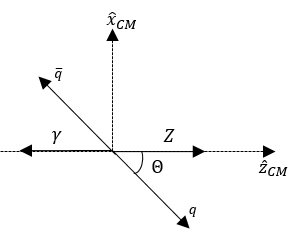
\includegraphics[width=0.3\textwidth]{fig/MVA/HZg_angle2.png}
		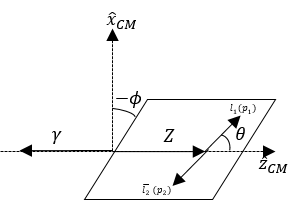
\includegraphics[width=0.3\textwidth]{fig/MVA/HZg_angle1.png}
	\end{center}
	\caption{Definitions of theoretical angles used for kinematic BDT training. The left diagram is in the Higgs boson center-of-mass frame, and the right diagram is in the $\PZ$ boson center-of-mass frame.}
	\label{fig:kinangles}
\end{figure}

\begin{figure}[tb]
	\begin{center}
		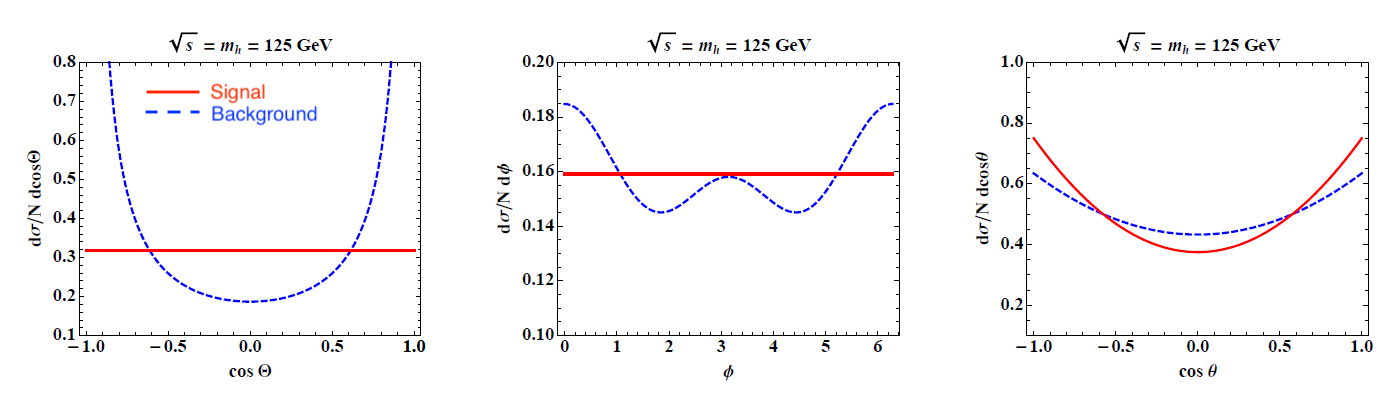
\includegraphics[width=0.9\textwidth]{fig/MVA/Zg_theorist.png}
		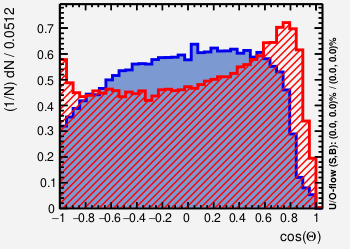
\includegraphics[width=0.3\textwidth]{fig/MVA/cosTheta_reco.png}
		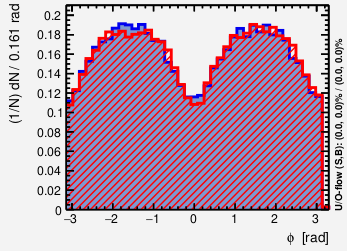
\includegraphics[width=0.3\textwidth]{fig/MVA/phi_reco.png}
		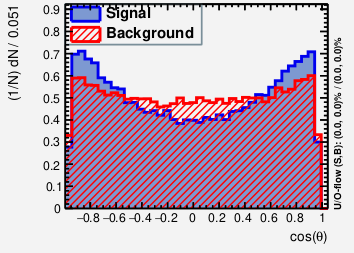
\includegraphics[width=0.3\textwidth]{fig/MVA/costheta_reco.png}
	\end{center}
	\caption[Top: Expected theoretical shapees for the angular features used for kinematic BDT training. Bottom: Reconstructed shapes for these quantities after the \hzg{} selection requirements have been applied. Please note that the red and blue color conventions are reversed for the top and bottom plots.]
	{Top: Expected theoretical shapes~\cite{HZg_angle1} for the angular features used for kinematic BDT training. Bottom: Reconstructed shapes for these quantities after the \hzg{} selection requirements have been applied. Please note that the red and blue color conventions are reversed for the top and bottom plots.} \label{fig:kin_GEN_angles}
\end{figure}

Several fundamental kinematic quantities of the final state particles are also used as training features. These include the pseudorapidity of each lepton, the $\Delta R$ between each lepton and the photon, and the $\pt/m$ of the $\lplm\gamma$ system. We note that the \pt values of each final state particle were also considered for training, but were found to have a negligible impact on discrimination power. This is likely because they are highly correlated with these other fundamental kinematic quantities, and thus, do not introduce much additional information to the BDT model. A comparison between signal and background shapes for these kinematic features is shown in Fig. \ref{fig:kin_training_shapes}.

\begin{figure}[tb]
	\begin{center}
		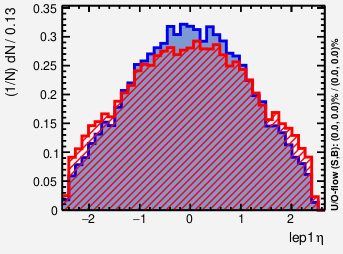
\includegraphics[width=0.3\textwidth]{fig/MVA/lepeta1_reco.png}
		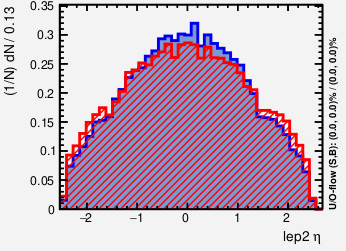
\includegraphics[width=0.3\textwidth]{fig/MVA/lepeta2_reco.png}
		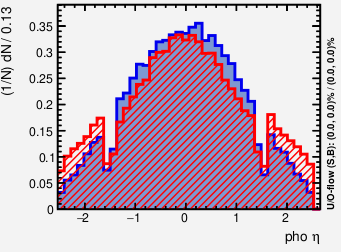
\includegraphics[width=0.3\textwidth]{fig/MVA/phoeta_reco.png}
		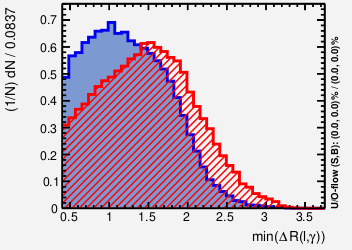
\includegraphics[width=0.3\textwidth]{fig/MVA/mindr_reco.png}
		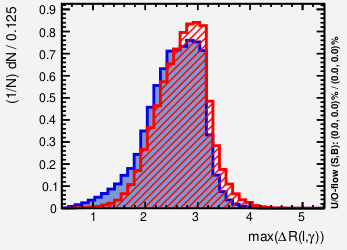
\includegraphics[width=0.3\textwidth]{fig/MVA/maxdr_reco.png}
		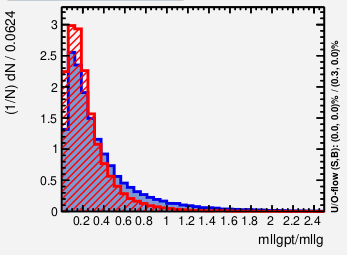
\includegraphics[width=0.3\textwidth]{fig/MVA/pt_over_m_reco.png}
	\end{center}
	\caption{Comparison of reconstructed signal and background shapes for several kinematic variables used for kinematic BDT training.}
	\label{fig:kin_training_shapes}
\end{figure}



The following features are used in the training of the kinematic BDT: photon MVA score, photon energy resolution, $\eta$ of each 
lepton and the photon, smallest and largest of the two $\Delta R$ values of the photon with respect to each lepton, $p_{T}/m$ for the 
three body system, and three theoretically motivated decay angles. The angular quantities are defined in Figure [FIG] and their 
theoretical, generator-level, and reconstructed distributions are shown in Figure [FIG]. The signal and background distributions
used in the training for all kinematic BDT features are shown in Figure [FIG]. Table [TAB] ranks the kinematic BDT 
training features in order of importance for the final discriminator. We observe that the most discriminating feature is the photon 
MVA identification score which mainly serves distinguish real photons from misreconstructed jets. A comparison of the BDT 
distributions in the training and test samples allows us to check for any possible overtraining of the model. This is shown in 
Figure [FIG], where no significant overtraining is observed. 

The output of the kinematic 
BDT in data and simulation is shown in Figure [FIG]. We observe good agreement between data and simulation. For additional 
validation of the method, two control regions are defined. A background-enriched control region is defined by 
$m_{\ell\ell} + m_{\ell\ell\gamma} < 185$ GeV or $p_{T}^{\gamma} < 15/110$, and an irreducible background-enriched (SM $Z\gamma$) 
control region is defince by $m_{\ell\ell} + m_{\ell\ell\gamma} < 185$ GeV and $80 < m_{\ell\ell} < 100$ GeV. The data and simulation
distributions for the kinematic BDT for these control regions are shown in Figures [FIGS]. Again, we observe good agreement 
between data and simulation.

\section{Vector Boson Fusion Boosted Decision Tree}
The dijet BDT is used to discriminate signal from VBF Higgs production from other dijet signal and background events. The training
and evaluation of the dijet BDT is only carried out on events which have two jets selected according to the requirements in 
section [SEC]. The training is performed using VBF \hzg events as signal and gluon-gluon fusion \hzg, SM $Z\gamma$, Z plus jets, and 
$t\bar{t}$ events as background. VH and ttH \hzg events are neglected, as their contribution is negligibly small. Only about 65\% 
of the signal jets correspond to the true VBF jets in which we are interested. Because of this, we perform an additional matching 
procedure for these jets. In order for an event to be used in the training, both reconstructed jets must be matched 
to generator-level partons, which must also be matched to the generator-level \pt values of the true VBF partons. As with the 
kinematic BDT, only half of the simulated events are used for the training procedure, with the remainder used for category optimization
and signal modeling. Again, events from all data-taking years in both the muon and electron channels are combined for the training. 
The samples are weightd by their respective cross sections and weighted by the luminosity of each year. 

The input features to the dijet BDT training include 
$\Delta\eta$(j, j), $\Delta\phi$(j, j), $\Delta\phi$($Z\gamma$, jj),  
$\Delta R(j,\gamma)$, ${p_{T}}^{j1,2}$,
$p_{T}^{t}$ (defined as $\frac{2|p_{Tx}^{Z}p_{Ty}^{\gamma}-p_{Ty}^{Z}p_{Tx}^{\gamma}|}{p_{T}^{H}}$),
system \pt balance (defined as 
$|\frac{\sum_{Z,\gamma,j_{1},j_{2}}{\vec{p}_{transverse}}^{i}}{\sum_{Z,\gamma,j_{1},j_{2}}p_{T}}|$),
photon Zeppenfeld variable (defined as $|\eta_{\gamma}-\frac{\eta_{j1}+\eta_{j2}}{2}|$), and
kinematic MVA score. The angular quantities provide discrimination between VBF and non-VBF events,
while the kinematic MVA score and $p_{T}^{t}$ provide discrimination between signal and 
background events. The $p_{T}^{t}$ [REF] is the component of the transverse momentum of the Z$\gamma$ system that
is perpendicular to the difference of the 3-momenta of the Z boson and the photon candidate. 


\section{Categorization Procedure}

The procedure used for event categorization is described below. 

\begin{enumerate}
  \item Events with at least one additional electron or muon with $\pt>7$ ($5$)\GeV are assigned to 
	  the lepton-tagged category.
  \item Events not assigned to the lepton-tagged category, but which contain two jets satisfying the 
	  selection requirements described in Section \ref{sec:selection}, are classified 
	  as dijet events, indicative of possible VBF production. If multiple dijet pairs exist within an event, the two jets with highest 
	  $\pt$ are considered. The subdivision of dijet events into a set of three dijet categories 
	  is described later in this section.
	  The VBF BDT classifier is trained to separate VBF signal events from $\Pg\Pg\PH$+jets and background events. 
  The distribution of $\mathcal{D}_{\mathrm{VBF}}$ is shown in Fig.~\ref{fig:BDT} (left) for both simulated event samples and data. 
  \item Events not assigned to the lepton-tagged or dijet categories are classified as untagged events.
	The subdivision of untagged events into a set of four untagged categories is described 
	later in this section.
  The kinematic BDT classifier is trained to distinguish signal events from background events based on the kinematics of the leptons and photon in the $\PZ\gamma$ candidate system, as well as on the measured properties of these physics objects.
  The distribution of $\mathcal{D}_{\mathrm{kin}}$ is shown in Fig.~\ref{fig:BDT} (right) for both simulated samples and data. 
\end{enumerate}

\begin{figure}[tbp!]
\centering
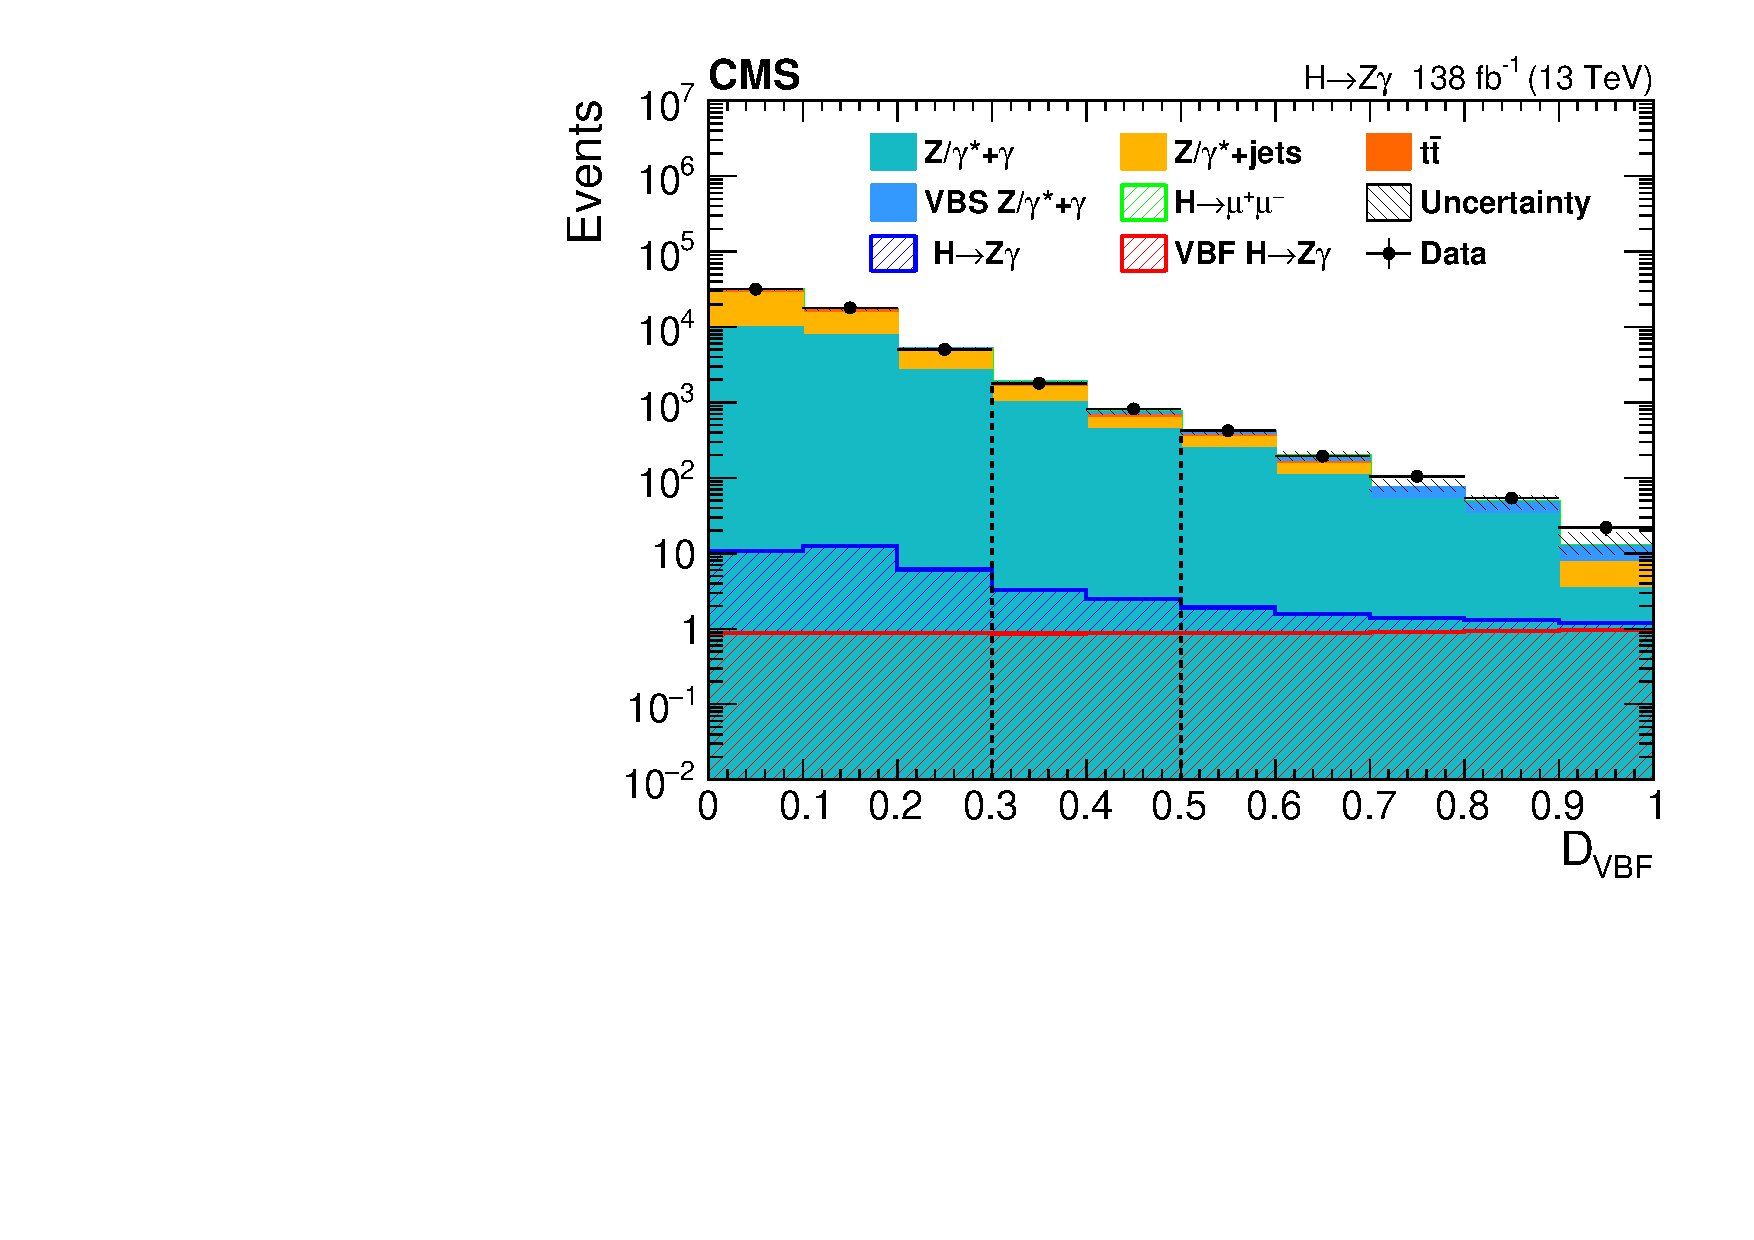
\includegraphics[width=0.47\textwidth]{fig/bdt/Figure_002-a.pdf}
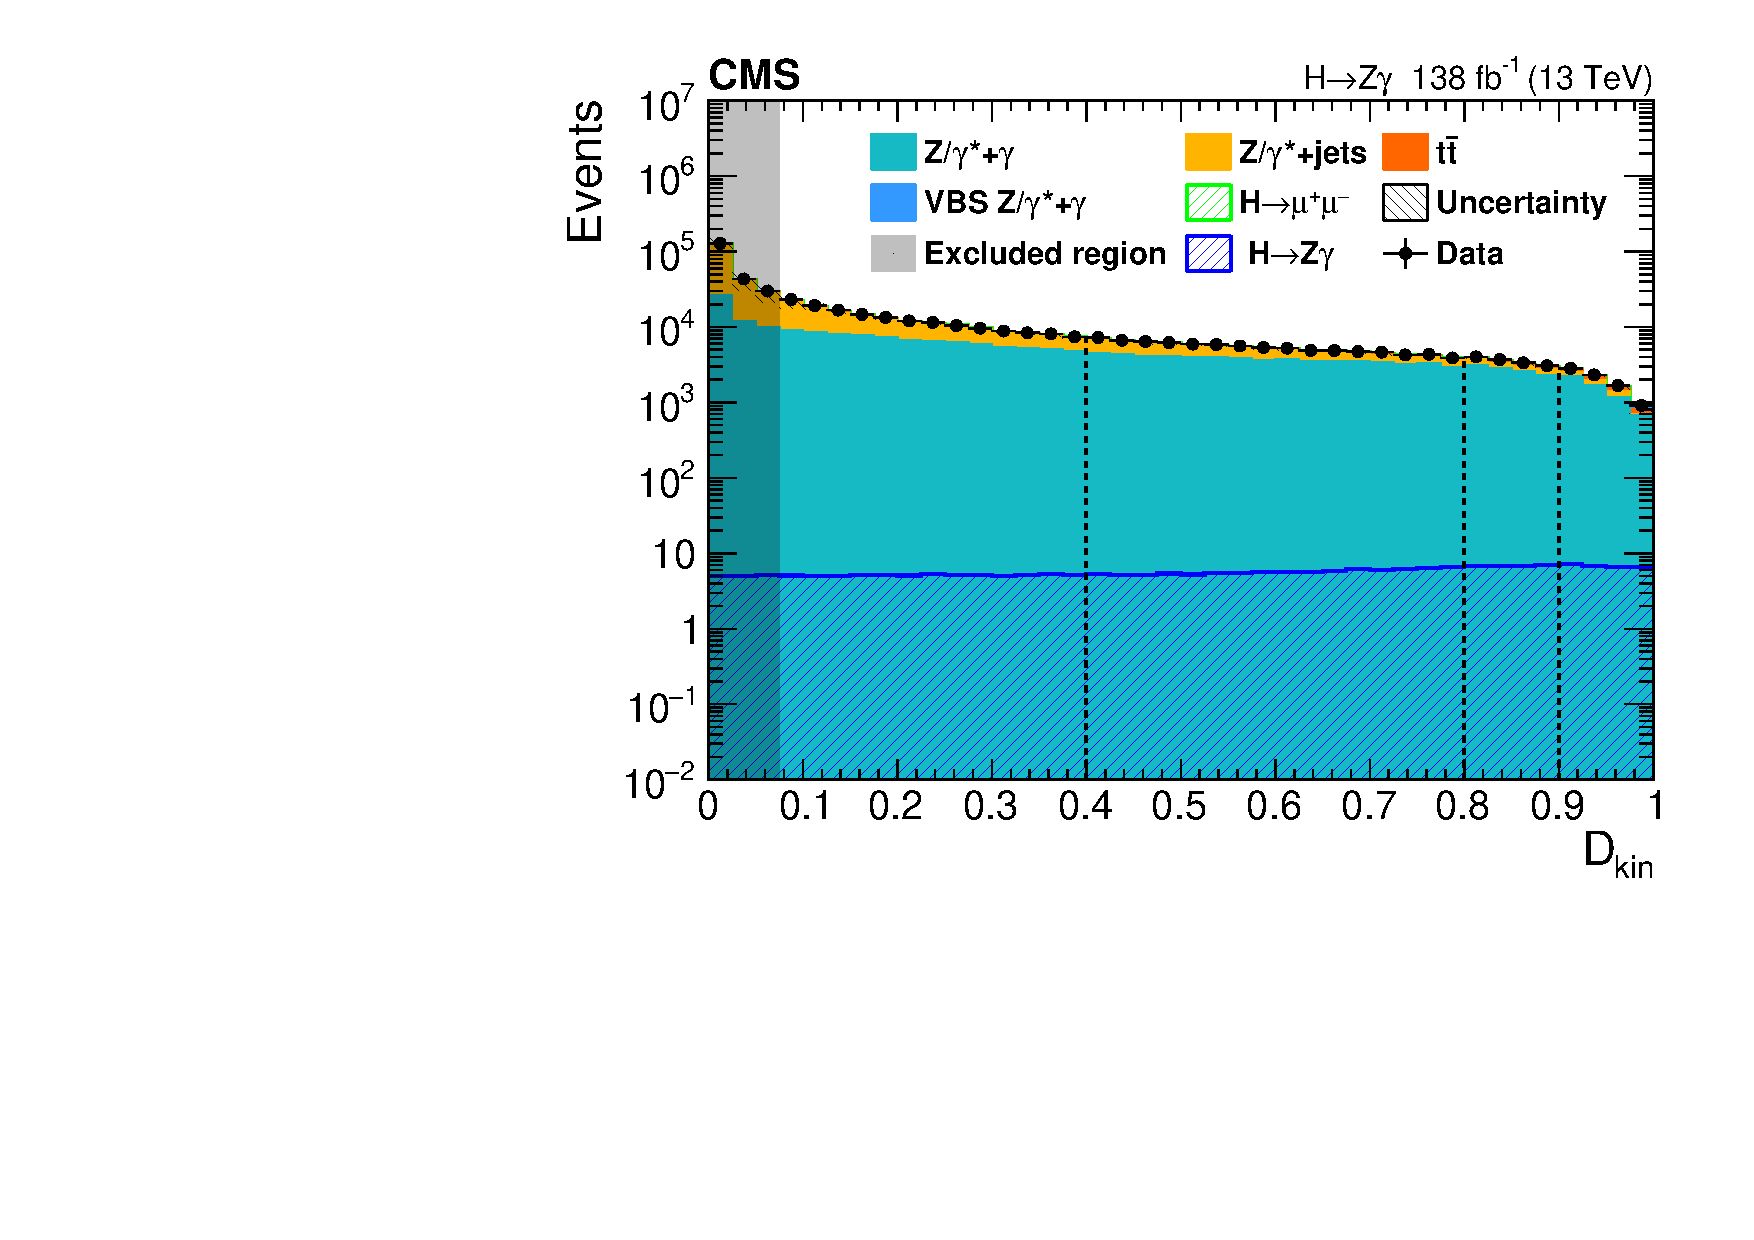
\includegraphics[width=0.47\textwidth]{fig/bdt/Figure_002-b.pdf}
 \caption{The $\mathcal{D}_{\mathrm{VBF}}$ (left) and $\mathcal{D}_{\mathrm{kin}}$ (right) distributions for signal, simulated background, and data. 
	  The $\mathcal{D}_{\mathrm{VBF}}$ distribution includes
	  only dijet-tagged events, and the $\mathcal{D}_{\mathrm{kin}}$ distribution includes only untagged events. The sum of contributions from all signal production mechanisms is shown by the blue line, while the contribution from only the VBF mechanism is shown by the red line. The uncertainty band incorporates all statistical and systematic uncertainties in the expected background. The dashed lines indicate the boundaries for the dijet and untagged categories. The gray shaded region in the $\mathcal{D}_{\mathrm{kin}}$ distribution is excluded from the analysis.\label{fig:BDT}}
\end{figure}

The subdivision of dijet and untagged events into categories is based on the VBF BDT and kinematic BDT discriminants.
Category boundaries are defined as mutually exclusive regions of $\mathcal{D}_{\mathrm{VBF}}$ and $\mathcal{D}_{\mathrm{kin}}$. 
The locations of the boundaries defining the categories are optimized by iterating over all possible combinations of boundaries using $\sum_{i}^{n} {S_i}^2/B_i$
as a figure-of-merit. The variables $S_i$ and $B_i$
represent the number of expected signal and background events in the ${i}^{th}$  
category, and $n$ is the total number of categories. 
We consider categories with boundaries corresponding to signal efficiencies  
between $0$--$100$\% in $10$\% increments.
The optimization procedure results in three dijet categories for the VBF BDT and four untagged categories for the kinematic BDT.
The lowest $\mathcal{D}_{\mathrm{kin}}$ boundary corresponds to the $10$\% point in integrated signal efficiency, 
and events below the $10$\% point are excluded from the analysis to preserve the stability of the background model.

The full categorization and optimization procedure results in the following eight mutually exclusive categories: 
one lepton-tagged category, three dijet categories, and four untagged categories. 
The category definitions are summarized in Table~\ref{tab:category}.
\begin{table}[!tb]
    \centering   
    \caption{Summary of the category definitions. The lepton-tagged category requires at least one additional electron or muon. Dijet categories are defined by regions of $\mathcal{D}_{\mathrm{VBF}}$ 
	  and untagged categories are defined by regions of $\mathcal{D}_{\mathrm{kin}}$.}
  \label{tab:category}
  \begin{tabular}{c@{\hskip 0.3in}ccc@{\hskip 0.3in}cccc}
    \hline
                 Lepton   & Dijet 1 & Dijet 2 & Dijet 3& Untagged 1 & Untagged 2 & Untagged 3 & Untagged 4 \\\hline
		  \multirow{2}{*}{$\geq$ 1 $\Pe,\mu$} &\multicolumn{3}{c}{$\mathcal{D}_{\mathrm{VBF}}$ selection}&\multicolumn{4}{c}{$\mathcal{D}_{\mathrm{kin}}$ selection}\\
        &0.5--1.0&0.3--0.5&0.0--0.3&0.9--1.0&0.8--0.9&0.4--0.8&0.1--0.4\\
        \hline
  \end{tabular}
\end{table}

Table~\ref{tab:yield} lists the event categories used in the analysis, along with the expected event yields for an $m_\PH=\mH\GeV$  signal arising from 
$\Pg\Pg\PH$, VBF, $\mathrm{V}\PH$, and $\ttbar\PH$ production, as well as a 6\% resonant background contribution from FSR from $\PH\rightarrow\Pgmp\Pgmm$. The expected event yield from $\PH\to\tau^+\tau^-$ is estimated to be below the 1\% level relative to the $\PH\to\PZ\gamma$ yield and is neglected.
The dominant contribution to the signal yield is generally from $\Pg\Pg\PH$ production, except in the lepton-tagged category, in which $\mathrm{V}\PH$ and $\ttbar\PH$ events dominate, and in the dijet 1 category, in which VBF events dominate.
The categorization procedure increases the sensitivity of the analysis by 24\% with respect to an inclusive event selection.  
The product of signal acceptance and efficiency for $\Pp\Pp\to\PH\to \PZ\gamma\to\ell^+\ell^-\gamma$ for $m_{\PH} =\mH\GeV$ is $23$ ($29$)\% in the electron (muon) channel.    

  \begin{table}[tb!]
    \centering   
	  \scriptsize
    \caption{Yields and approximate significance ($S/\sqrt{B}$) for each category, where $S$ and $B$ are the expected number of signal and background events in the narrowest $m_{\ell^+\ell^-\gamma}$ interval containing 95\% of the expected signal distribution.
    Also shown is the $m_{\ell^{+}\ell^{-}\gamma}$ resolution, computed using the narrowest interval containing 68\% of the expected signal distribution. 
	   }
  \begin{tabular}{c@{\hskip 0.3in}ccccccccc}
    \LumiT\fbinv   & Lepton   &  & Dijet 1 & Dijet 2 & Dijet 3& Untagged 1 & Untagged 2 & Untagged 3 & Untagged 4\\\hline
  \tabincell{c}{\textbf{SM signal}\\\textbf{yield}}    &&        &           &           &           &        &        &        &       \\
  $\Pg\Pg\PH$             & 0.51   & \tabincell{c}{$\Pe^+\Pe^-$\\$\mu^+\mu^-$} & \tabincell{c}{1.10\\1.41}& \tabincell{c}{1.62\\2.05}& \tabincell{c}{9.44\\12.1}&\tabincell{c}{6.89\\8.52}& \tabincell{c}{7.35\\9.17}& \tabincell{c}{29.8\\38.0}&\tabincell{c}{22.5\\29.0}\\
  &        &           & &           &           &        &        &        &       \\
  VBF             & 0.09   & \tabincell{c}{$\Pe^+\Pe^-$\\$\mu^+\mu^-$}& \tabincell{c}{1.94\\2.40}& \tabincell{c}{0.76\\0.97}&  \tabincell{c}{1.13\\1.43}& \tabincell{c}{0.71\\0.89}& \tabincell{c}{0.35\\0.43}& \tabincell{c}{0.92\\1.18}& \tabincell{c}{0.51\\0.65}\\
  &        &           & &           &           &        &        &        &       \\
  $\mathrm{V}\PH+\ttbar\PH$& 1.84  & \tabincell{c}{$\Pe^+\Pe^-$\\$\mu^+\mu^-$} & \tabincell{c}{0.04\\0.05}& \tabincell{c}{0.13\\0.16}& \tabincell{c}{1.89\\2.36}& \tabincell{c}{0.31\\0.39}& \tabincell{c}{0.17\\0.21}& \tabincell{c}{0.45\\0.57}& \tabincell{c}{0.27\\0.33}\\\hline
  \tabincell{c}{\textbf{SM resonant} \\\textbf{background}}&&&&&&&&&\\
  $\PH\rightarrow\mu^+\mu^-$     & 0.14& $\mu^+\mu^-$&0.27 & 0.27 & 0.43& 0.62& 0.49 & 2.02& 1.78\\\hline
 
  \tabincell{c}{\textbf{Mass} \\\textbf{resolution}\\(GeV)} & 2.12& \tabincell{c}{$\Pe^+\Pe^-$\\$\mu^+\mu^-$}& \tabincell{c}{1.91\\1.52}& \tabincell{c}{2.06\\1.61}& \tabincell{c}{2.15\\1.72}& \tabincell{c}{1.80\\1.37}& \tabincell{c}{1.97\\1.42}& \tabincell{c}{2.12\\1.62}& \tabincell{c}{2.33\\1.83}\\
  \hline
  
  \textbf{Data yield}            & 1485   && 168    & 589    & 11596& 1485      & 1541      & 2559      & 17608   \\\hline
  \textbf{$S/\sqrt{B}$}    & 0.06  && 0.54  & 0.24  & 0.26& 0.45  & 0.35  & 0.53  & 0.30  \\
  
  \\
  \end{tabular}
  \label{tab:yield}
  \end{table}

\section{Dropping of Boosted Category}

In the previous 2016 analysis, a boosted Higgs category was used. This category is defined by a simple cut on the \pt of the
$\ell\ell\PGg$ system.
However, for the current MVA-based analysis, the Higgs kinematics 
are already included in the BDT training. In this case, it stands to reason that the boosted category may no longer be useful for 
improving the analysis senstivity. We therefore test the possibility of constructing a boosted category before constructing the 
untagged categories to see whether the combined significance is increased or decreased.
The left plot of Figure \ref{fig:llgpt} shows the \pt spectrum of the $\ell\ell\PGg$ system for various signal MC samples. 
We see that the \pt spectrum for the gluon-gluon fusion process is similar to the main backgrounds, 
while the other signal processes are more boosted. 
The right plot shows the upper limit on $\sigma/\sigma_{SM}$ as a function of a \pt cut on the $\ell\ell\PGg$ system,
where the background estimation is taken from data. 
The upper limit for the boosted category (shown in blue) worsens as the \pt cut increases. This is expected since we lose 
a substantial amount of gluon-gluon fusion signal. However, the combined limit of the untagged categories improves.
The overall combined limit (shown in black) is rather flat as a function of the \pt of the $\ell\ell\PGg$ system. 
For the overall combined limit, we observe fluctuations beyond a \pt cut of 60 \GeV, so we choose 60 \GeV as the cut defining
a potential boosted category. Comparing the combined significance of the boosted category plus untagged categories to the 
untagged categories alone, we see that the combined significance is substantially higher for the untagged categories alone. An explanation for this behavior is as follows.
In the current analysis flow, dijet events are selected before boosted events. 
We loosen the dijet selection requirements, which causes the boosted events to migrate to the 
dijet categories and reduces the significance of boosted category.
Therefore, we choose not to use a boosted category in this version of the analysis. 
 \begin{figure}[htbp]
 	\begin{center}
 		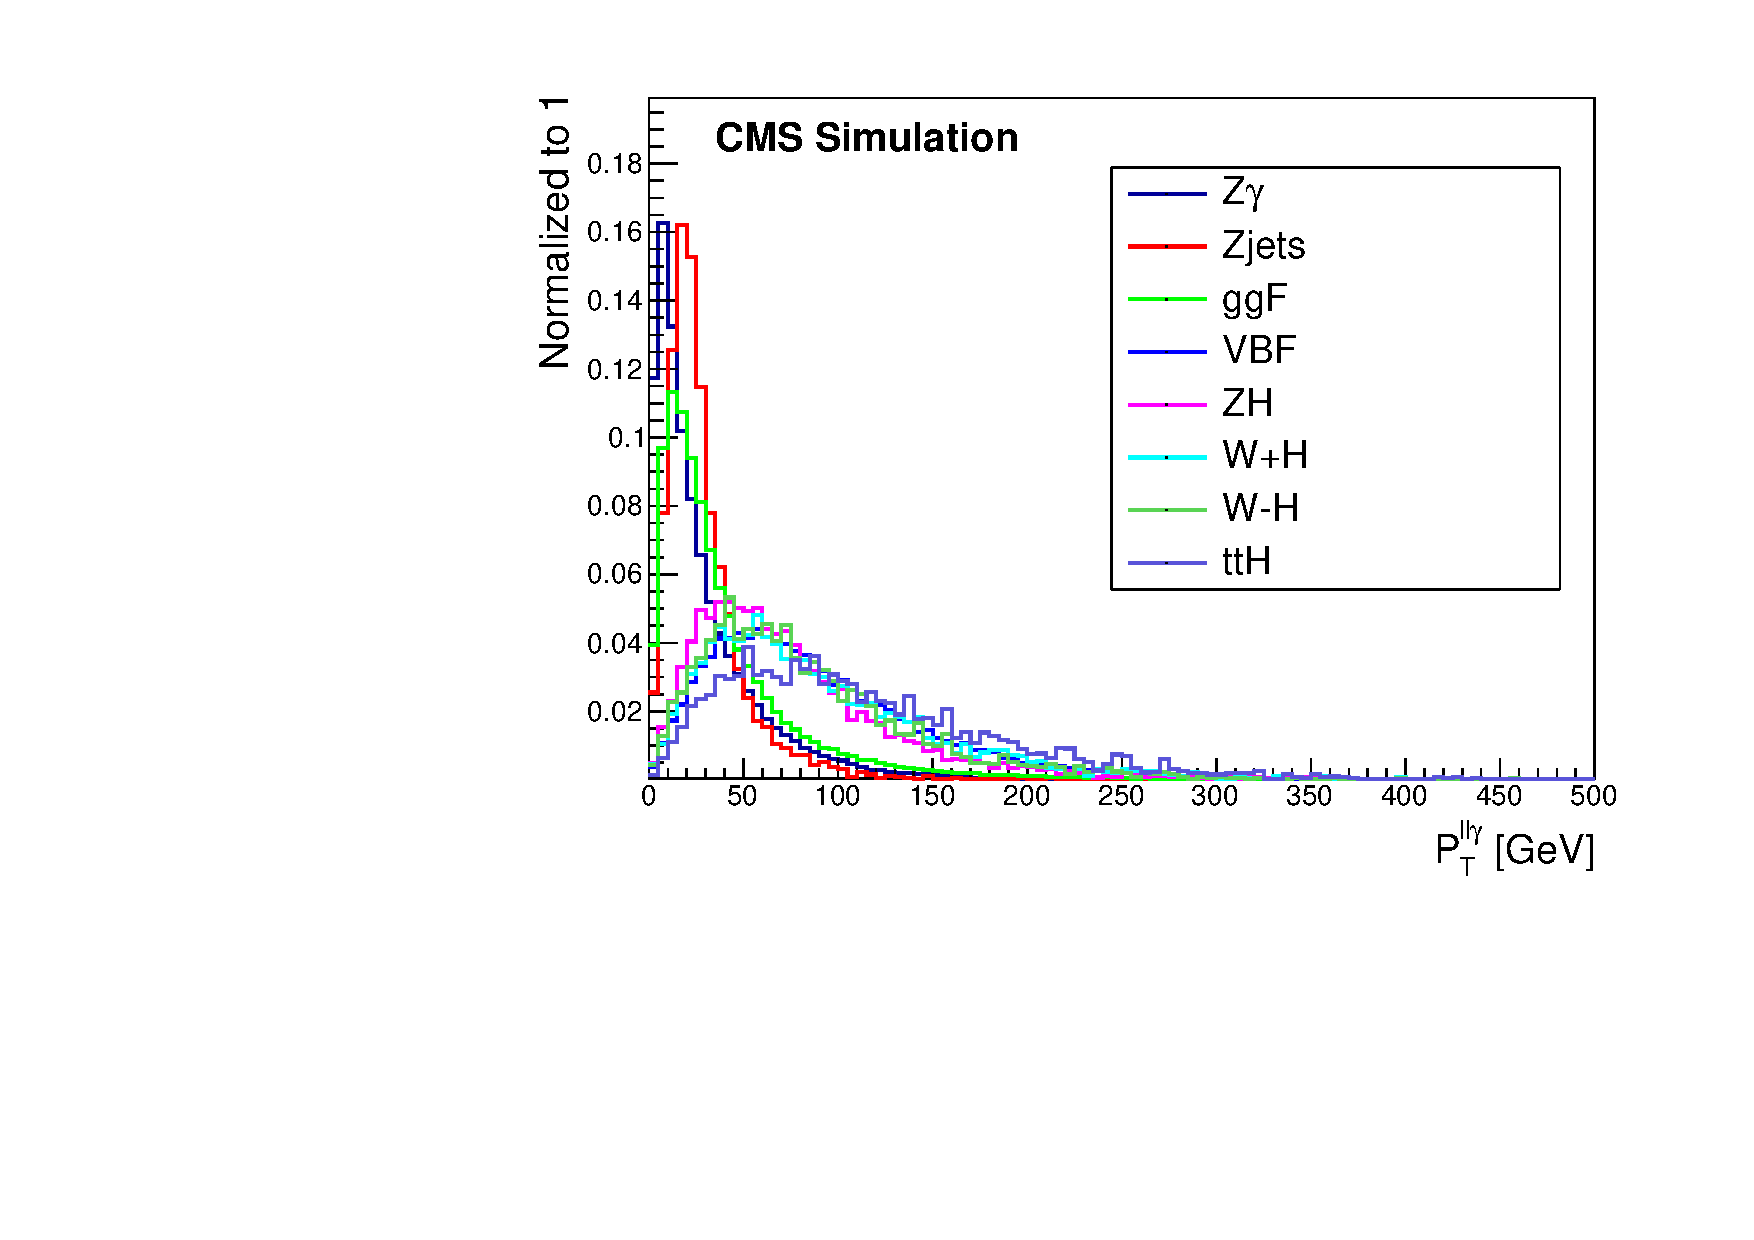
\includegraphics[width=0.4\textwidth]{fig/boosted/hptllg_inc_e.pdf}
 		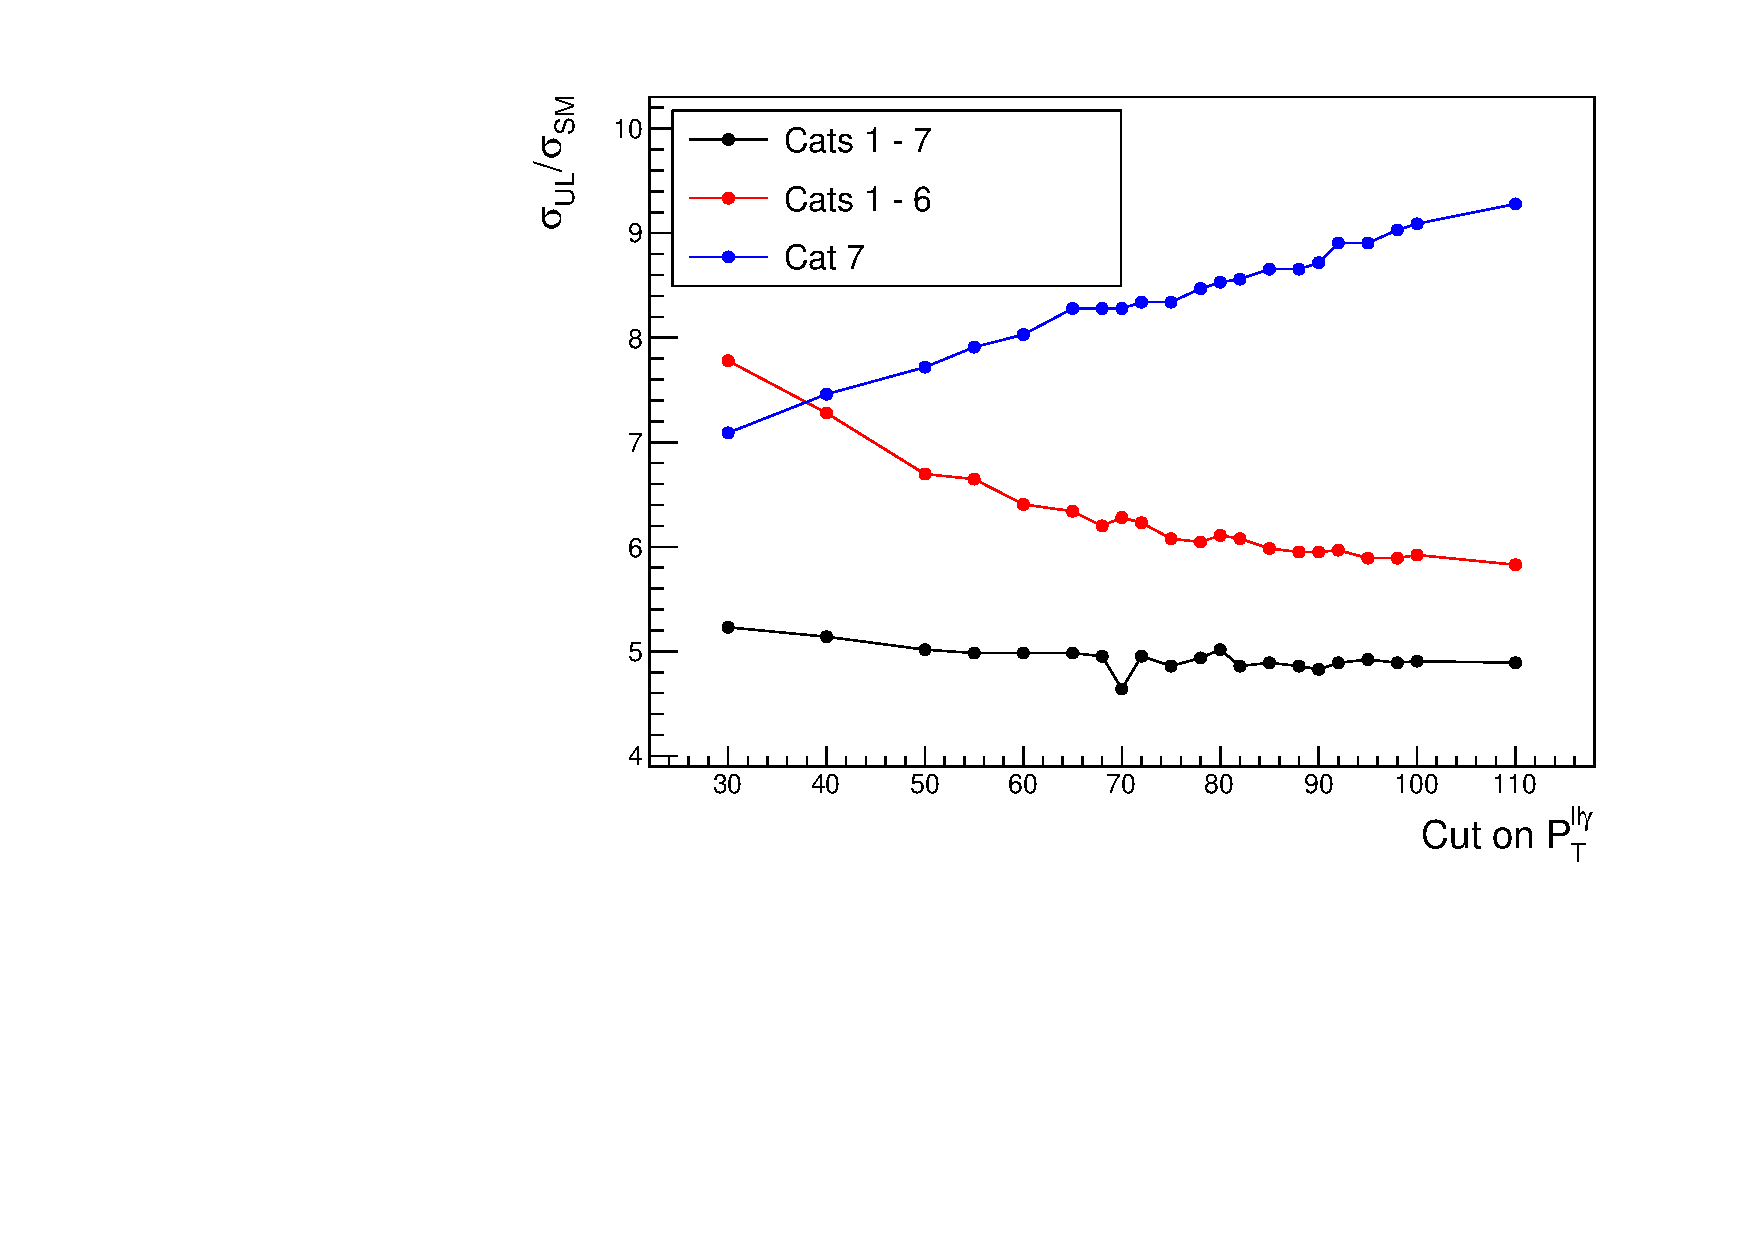
\includegraphics[width=0.4\textwidth]{fig/boosted/plot_opt_boostedcat.pdf}

 	\end{center}
 	\caption{Left: $\ell\ell\PGg$ \pt for different signal MC processes. Right: optimization of the boosted category by scanning the expected limit as function of $\ell\ell\PGg$ \pt.}
 	\label{fig:llgpt}
 \end{figure}
 \begin{figure}[htbp]
	\begin{center}
		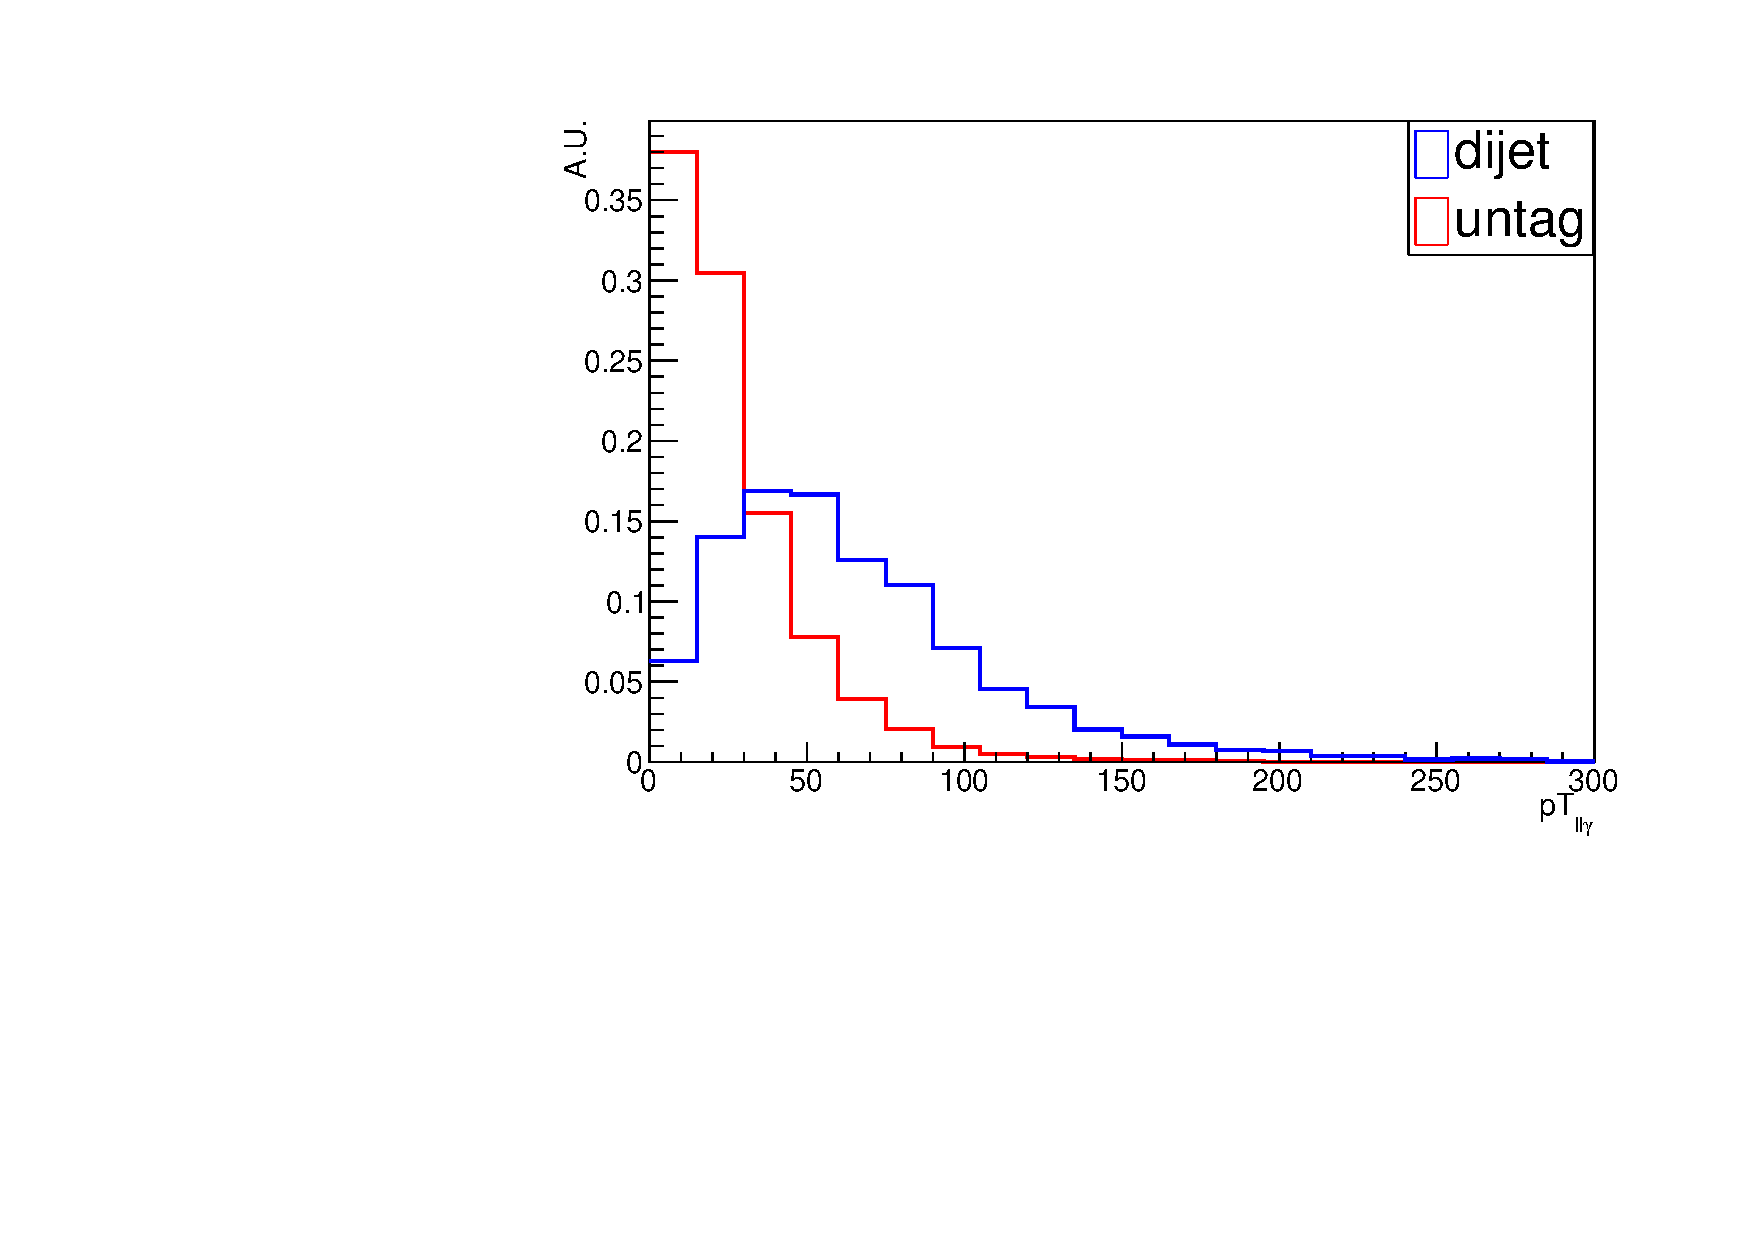
\includegraphics[width=0.4\textwidth]{fig/boosted/mllgpt_VBFuntag.pdf}
		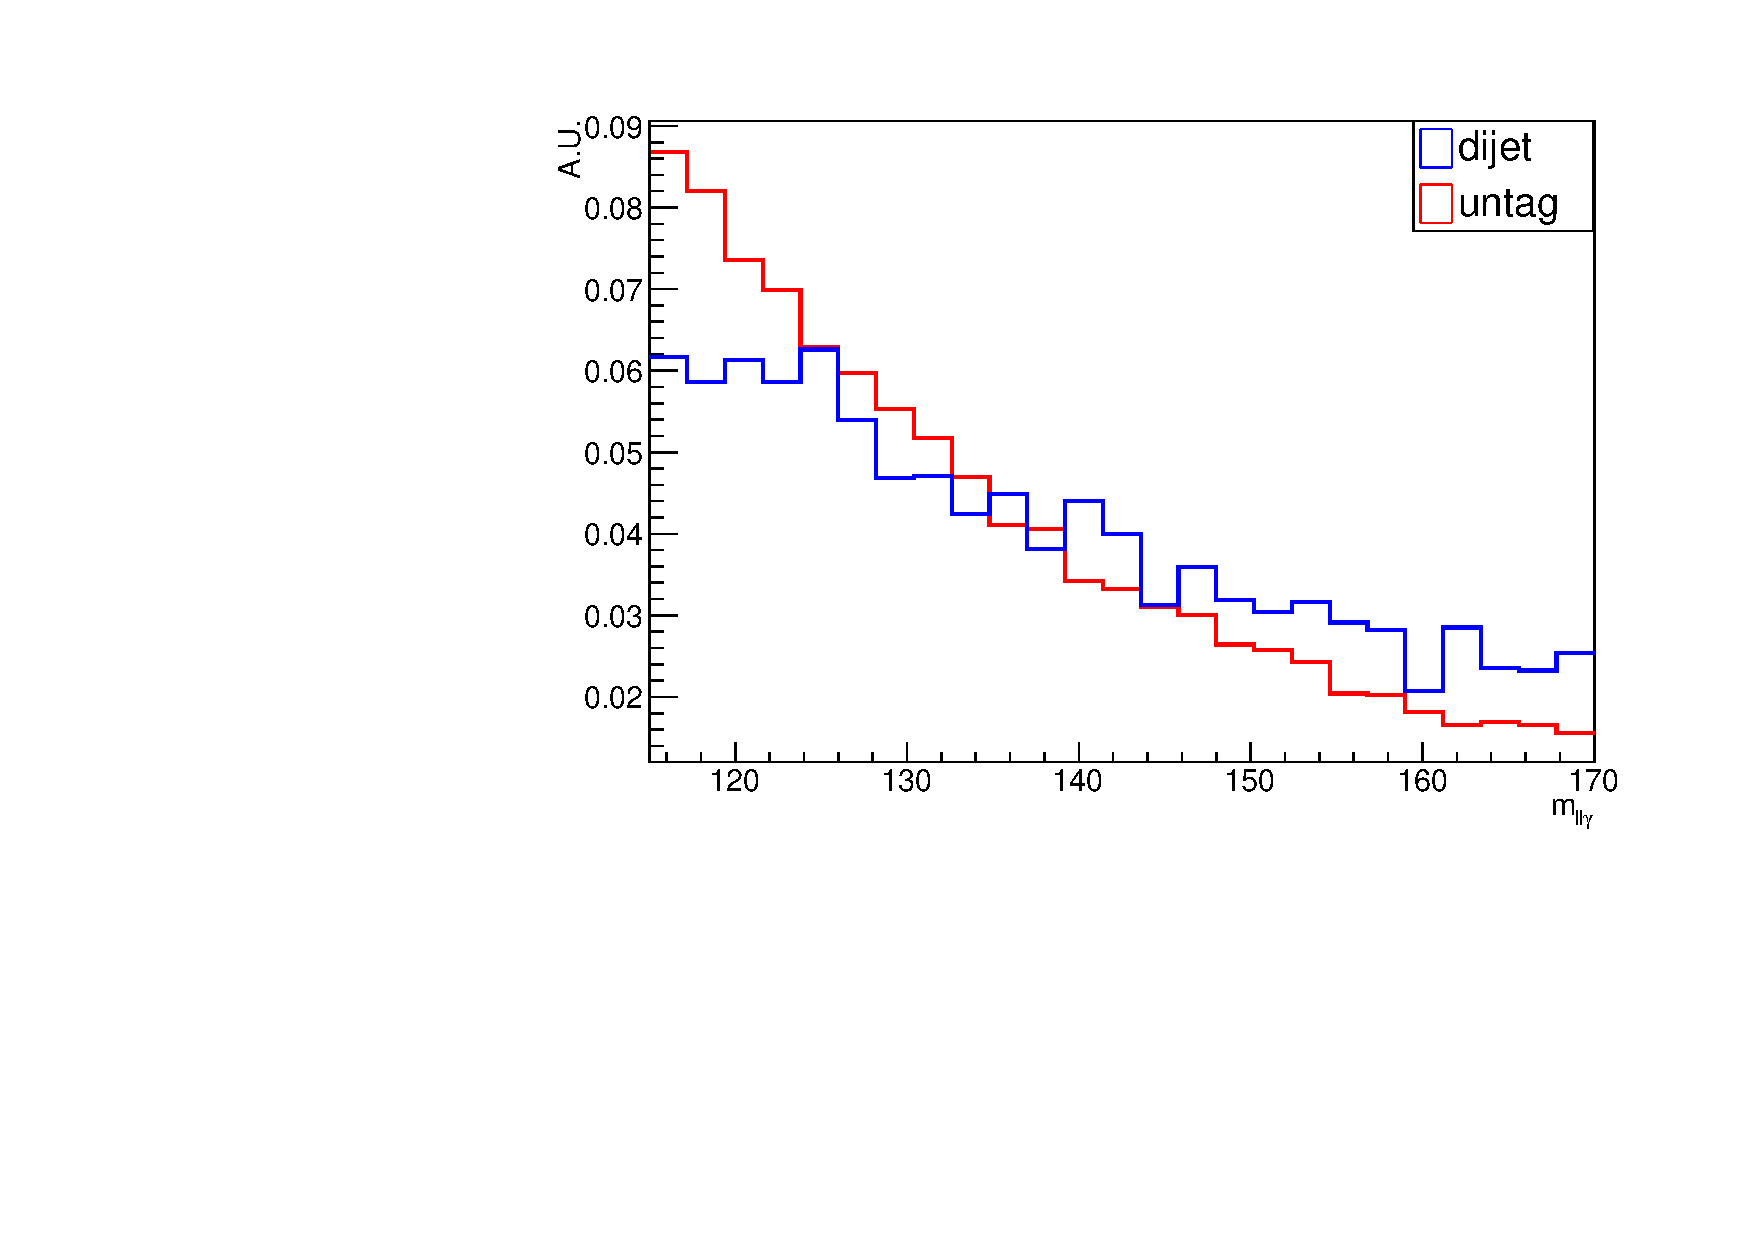
\includegraphics[width=0.4\textwidth]{fig/boosted/mllg_VBFuntag.pdf}
		
	\end{center}
	\caption{Left: $\ell\ell\PGg$ \pt for untagged events and dijet events. Right: The $m_{\ell\ell\PGg}$ spectrum of untagged events and dijet events.}
	\label{fig:dijetboost}
\end{figure}

